\vspace{2mm}
\begin{figure}[h!]
\tikzset{every picture/.style={line width=0.75pt}} %set default line width to 0.75pt        

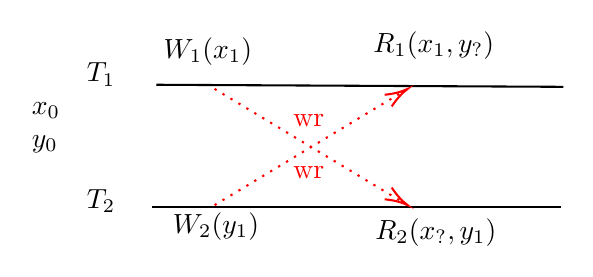
\begin{tikzpicture}[x=0.75pt,y=0.75pt,yscale=-1,xscale=1]
%uncomment if require: \path (0,300); %set diagram left start at 0, and has height of 300

%Straight Lines [id:da9500410641573396] 
\draw    (61.45,42) -- (257.56,43) ;
%Straight Lines [id:da7796185686481738] 
\draw    (59.56,101) -- (256.62,101) ;
%Straight Lines [id:da05192673528173475] 
\draw [color={rgb, 255:red, 255; green, 0; blue, 0 }  ,draw opacity=1 ] [dash pattern={on 0.84pt off 2.51pt}]  (89.56,100) -- (180.85,45.03) ;
\draw [shift={(182.56,44)}, rotate = 148.95] [color={rgb, 255:red, 255; green, 0; blue, 0 }  ,draw opacity=1 ][line width=0.75]    (10.93,-3.29) .. controls (6.95,-1.4) and (3.31,-0.3) .. (0,0) .. controls (3.31,0.3) and (6.95,1.4) .. (10.93,3.29)   ;
%Straight Lines [id:da10349511339666284] 
\draw [color={rgb, 255:red, 255; green, 0; blue, 0 }  ,draw opacity=1 ] [dash pattern={on 0.84pt off 2.51pt}]  (89.56,44) -- (180.85,98.97) ;
\draw [shift={(182.56,100)}, rotate = 211.05] [color={rgb, 255:red, 255; green, 0; blue, 0 }  ,draw opacity=1 ][line width=0.75]    (10.93,-3.29) .. controls (6.95,-1.4) and (3.31,-0.3) .. (0,0) .. controls (3.31,0.3) and (6.95,1.4) .. (10.93,3.29)   ;

% Text Node
\draw (26.5,30) node [anchor=north west][inner sep=0.75pt]   [align=left] {$T_1$};
% Text Node
\draw (26.5,91) node [anchor=north west][inner sep=0.75pt]   [align=left] {$T_2$};
% Text Node
\draw (165.56,105) node [anchor=north west][inner sep=0.75pt]   [align=left] {$R_2(x_?,y_1)$};
% Text Node
\draw (63.56,18) node [anchor=north west][inner sep=0.75pt]   [align=left] {$W_1(x_1)$};
% Text Node
\draw (68,102) node [anchor=north west][inner sep=0.75pt]   [align=left] {$W_2(y_1)$};
% Text Node
\draw (164.56,15) node [anchor=north west][inner sep=0.75pt]   [align=left] {$R_1(x_1,y_?)$};
% Text Node
\draw (0,49) node [anchor=north west][inner sep=0.75pt]   [align=left] {$x_0 $\\ $y_0$};

\draw (126,55) node [anchor=north west][inner sep=0.75pt]  [color={rgb, 255:red, 255; green, 0; blue, 0 }  ,opacity=1 ] [align=left] {wr};

\draw (126,80) node [anchor=north west][inner sep=0.75pt]  [color={rgb, 255:red, 255; green, 0; blue, 0 }  ,opacity=1 ] [align=left] {wr};
\end{tikzpicture}
\caption{G-1b cycle between $T_1$ and $T_2$, (wr, wr)}
\end{figure}
\vspace{2mm}
\begin{equation}
History\ H: [W_1(x_1),W_2(y_1),R_1(x_1),R_1(y_?),R_2(x_?),R_2(y_1),C_1, C_1]
\end{equation}
\vspace{2mm}